\section{Model: Linear Discriminant Analysis (LDA)}

\subsection{Introduction}
Linear Discriminant Analysis (LDA) is a classification algorithm that models the difference between classes by projecting data onto a lower-dimensional space that maximizes class separability. While LDA is often used as a dimensionality reduction technique, it differs significantly from methods like PCA. Notably:

\begin{itemize}
    \item \textbf{LDA is a supervised learning method}, meaning it utilizes label information during the projection. In contrast, \textbf{PCA is unsupervised} and does not take class labels into account when identifying principal components.
    
    \item \textbf{LDA reduces the data to at most $(C - 1)$ dimensions}, where $C$ is the number of classes. For binary classification, this means the data is reduced to just one dimension. This limitation makes LDA unsuitable as a general-purpose dimensionality reduction method for high-dimensional feature spaces.
    
    \item \textbf{PCA focuses on preserving variance}, finding directions that capture the most information in terms of spread, regardless of class structure. In contrast, \textbf{LDA explicitly finds directions that maximize class separability}.
\end{itemize}

\textbf{Conclusion:} Due to the limitations above, particularly the constraint on output dimensionality and its dependence on class labels, LDA was not used for dimensionality reduction in our experiments. Instead, we treated LDA as a dedicated classifier, alongside models such as Decision Tree and Naive Bayes.

\subsection{Training Configuration}
The LDA model was trained using a grid search over the following hyperparameters:

\begin{itemize}
    \item \textbf{Solver}: \texttt{lsqr}, \texttt{eigen}
    \item \textbf{Shrinkage}: \texttt{None}, \texttt{auto} (only applicable with \texttt{lsqr} or \texttt{eigen})
    \item \textbf{Tolerance (tol)}: \texttt{1e-4}, \texttt{1e-3}, \texttt{1e-2}
\end{itemize}

The best hyperparameters selected were:
\begin{itemize}
    \item \textbf{Solver}: \texttt{lsqr}
    \item \textbf{Shrinkage}: \texttt{None}
    \item \textbf{Tolerance}: \texttt{1e-4}
\end{itemize}

\subsection{Training and Evaluation Results}
The model was trained and validated using K-Fold Cross-Validation with Count Vectorizer as the embedding method.

\textbf{Training Performance Metrics:}

\begin{table}[H]
    \centering
    \caption{Training Performance Metrics for LDA}
    \label{tab:lda-training-metrics}
    \begin{tabular}{|l|c|c|c|c|c|}
        \hline
        \textbf{Method} & \textbf{Accuracy} & \textbf{ROC AUC} & \textbf{F1} & \textbf{Precision} & \textbf{Recall} \\ 
        \hline
        Count Vectorizer & 0.74 & 0.74 & 0.76 & 0.73 & 0.80 \\ 
        \hline
    \end{tabular}
\end{table}

\textbf{Testing Performance Metrics:}

\begin{table}[H]
    \centering
    \caption{Testing Performance Metrics for LDA}
    \label{tab:lda-testing-metrics}
    \begin{tabular}{|l|c|c|c|c|c|}
        \hline
        \textbf{Method} & \textbf{Accuracy} & \textbf{ROC AUC} & \textbf{F1} & \textbf{Precision} & \textbf{Recall} \\ 
        \hline
        Count Vectorizer & 0.7539 & 0.8292 & 0.7724 & 0.7358 & 0.8129 \\ 
        \hline
    \end{tabular}
\end{table}

\textbf{Best Model Selection Criteria:}

\begin{itemize}
    \item Testing performance is the primary metric for selecting the best model.
    \item Selection priority is based on: Accuracy > F1 Score > ROC AUC.
    \item Based on these metrics, the best LDA configuration is:
\end{itemize}

\begin{verbatim}
{
    "method": "count",
    "model": "lda",
    "hyperparameters": { "solver": "lsqr", "shrinkage": None, "tol": 0.0001 },
    "performance": {
        "accuracy": 0.7539,
        "precision": 0.7358,
        "recall": 0.8129,
        "f1": 0.7724,
        "roc_auc": 0.8292
    }
}
\end{verbatim}

\subsection{Performance Analysis}
\begin{itemize}
    \item \textbf{Accuracy Analysis}: The LDA model with Count Vectorizer achieved a test accuracy of 75.39\%, comparable to Logistic Regression.
    
    \item \textbf{Loss Analysis}: Training and validation loss curves (see Figure~\ref{fig:lda-loss}) show convergence without significant overfitting.
    
    \item \textbf{ROC AUC}: The model demonstrates strong discriminative ability with an ROC AUC of 82.92\%.
    
    \item \textbf{Precision and Recall}: The classifier balanced false positives and false negatives well, with a precision of 73.58\% and recall of 81.29\%.
    
    \item \textbf{Model Viability}: Despite LDA's assumptions (e.g., multivariate normality and equal class covariances), the model performed competitively on this dataset.
\end{itemize}

\subsection{Visualization of Training Results}
\begin{figure}[H]
    \centering
    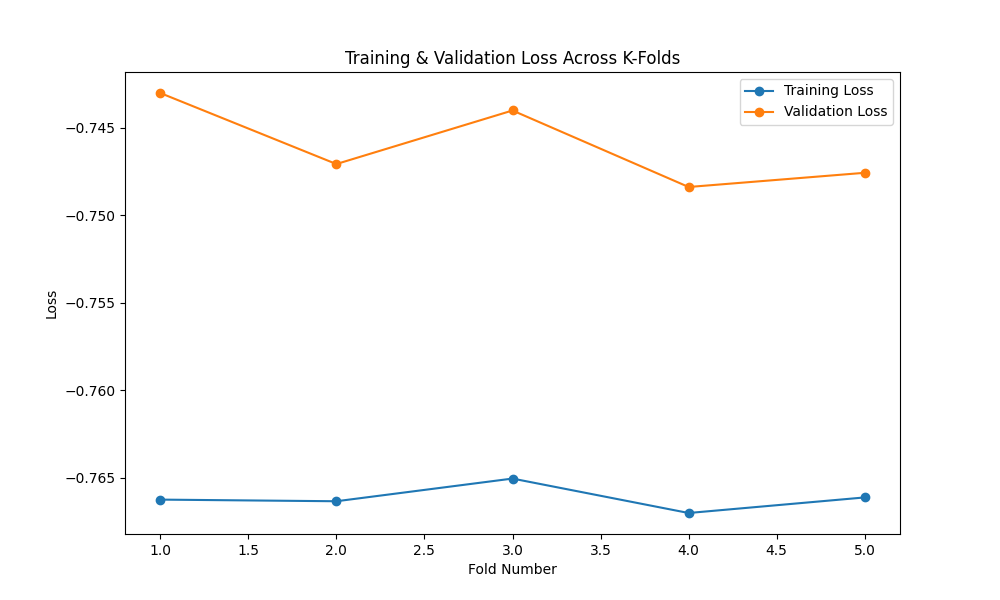
\includegraphics[width=0.7\textwidth]{img/report_info/img/9_2_LDA/best_lda_count_loss.png}
    \caption{Loss Curve - LDA with Count Vectorizer}
    \label{fig:lda-loss}
\end{figure}

\begin{figure}[H]
    \centering
    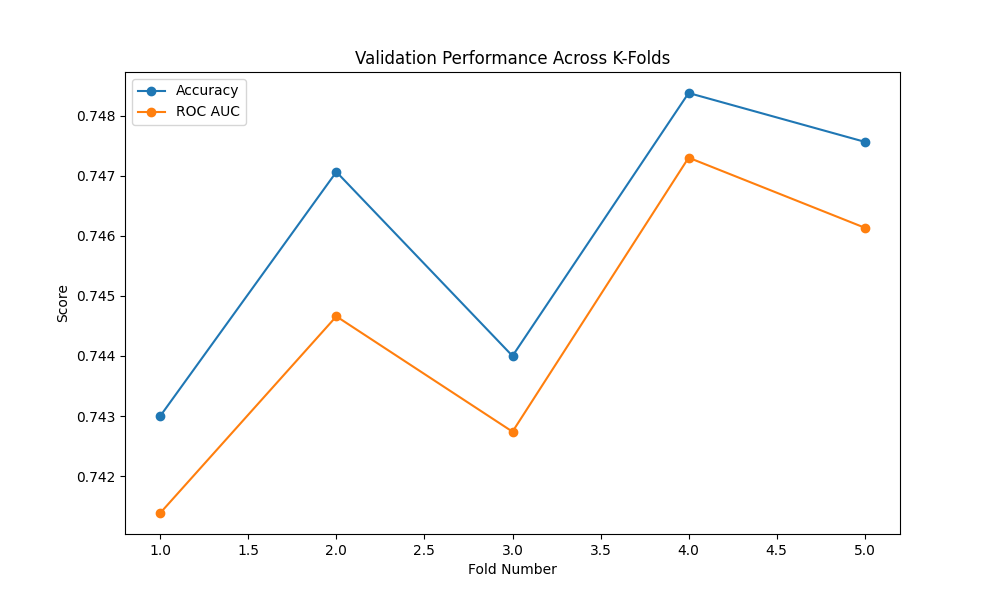
\includegraphics[width=0.7\textwidth]{img/report_info/img/9_2_LDA/best_lda_count.png}
    \caption{Performance Metrics - LDA with Count Vectorizer}
    \label{fig:lda-performance}
\end{figure}

\textbf{Image Description:}

\begin{itemize}
    \item \textbf{Loss Analysis}: The loss curve indicates a smooth and stable training process.
    \item \textbf{Validation Metrics}: Accuracy and ROC AUC remain stable across folds, indicating good generalization.
\end{itemize}

\subsection{Conclusion}

LDA, though often used for dimensionality reduction, is more appropriate here as a classifier due to the nature of binary classification. The method's inability to reduce to more than one dimension in binary settings, and its reliance on label information, makes it unsuitable for feature extraction like PCA.

Instead, the model was evaluated as a classifier and yielded strong results. With an accuracy of 75.39\% and ROC AUC of 82.92\%, the LDA model stands as a competitive alternative to Logistic Regression. It provides robust baseline classification performance using simple linear decision boundaries, especially when combined with Count Vectorizer features.
